\chapter{散乱角度} \label{cha:angle}
\section{光生成反応の散乱角度}
図のように$\mu,  \gamma^*N$系の散乱角$\theta, \phi$を定義する。\ref{fig:angle1}
\begin{figure}[H]
    \centering
    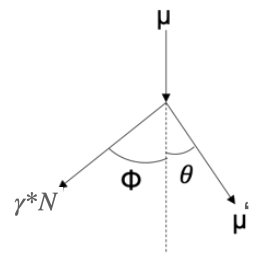
\includegraphics[width=8cm]{img/angle_diagram.png}
    \caption{散乱角$\theta, \phi$の定義}
    \label{fig:angle1}
\end{figure}

\subsection{$\theta$の考察}
下図のような運動学変数を考える。\ref{fig:angle2}
\begin{figure}[H]
    \centering
    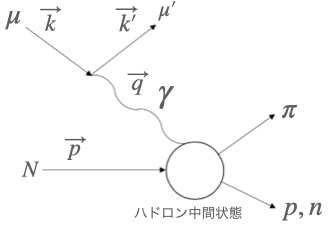
\includegraphics[width=8cm]{img/diagram_3momentum.png}
    \caption{運動学変数の定義}
    \label{fig:angle2}
\end{figure}

各値に対して以下のような定義を行う。
\begin{equation}
    \vec{k} = (E_\mu , p_\mu,0)
\end{equation}
\begin{equation}
    \vec{k'} = (E'_\mu, p'_\mu cos\theta, p'_\mu sin\theta)
\end{equation}
\begin{equation}
    \vec{p} = (m_N, 0, 0)
\end{equation}
\begin{equation}
    \vec{q} = k-k'=(E_\mu - E'_\mu, p_\mu-p'_\mu cos\theta, -p'_\mu sin\theta)
\end{equation}

また、$Q^2$は$\vec{q}$を用いることにより、以下のように表せる。
\begin{equation}
    Q^2 = -q^2 = 2E_\mu E'_\mu -2m^2_\mu-2p_\mu p'_\mu cos\theta
\end{equation}
これを$\theta$について解くと、$E'_\mu = E_\mu(1-y), p'_\mu = \sqrt{E'^2_\mu - m^2_\mu}$
を用いて$E'_\mu, p'_\mu$を消去すると、
\begin{eqnarray}
    \theta & = &\arccos{(\dfrac {2E_\mu E'_\mu -2m^2_\mu-Q^2}{2p_\mu p'_\mu})} \\
    & = & \arccos{(\dfrac{-Q^2-2m^2_\mu+2E^2_\mu(1-y)}{2\sqrt{E^2_\mu-p^2_\mu}\sqrt{E^2_\mu(1-y)^2-m^2_\mu} } )}
\end{eqnarray}
